\documentclass{math}

\usepackage{graphicx}
\usepackage{listings}

\title{Principles of Data Mining: HW 03}
\author{Alvin Lin}
\date{August 2018 - December 2018}
\begin{document}

\maketitle

\subsection*{Cost Functions (non-mixed)}
\begin{center}
  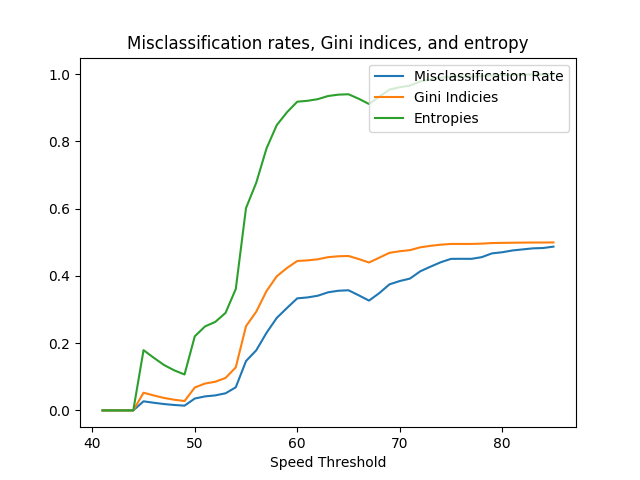
\includegraphics[width=16cm]{assets/hw_03_cost_functions.png}
\end{center}

\subsection*{Cost Functions (mixed)}
\begin{center}
  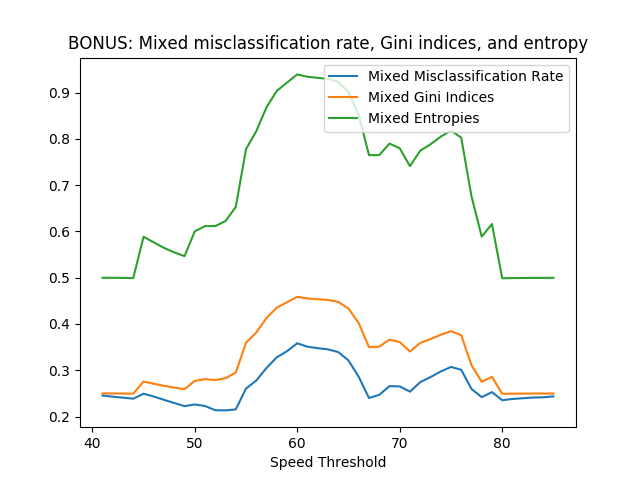
\includegraphics[width=16cm]{assets/hw_03_mixed_cost_functions.png}
\end{center}

\subsection*{Conclusion}
If we only account for the subset below the speed threshold, then the entropy
approaches 1 as we approach the highest speed threshold because at that point,
we have included all the data in consideration. In general, the cost function
approaches its maximum as we move towards the highest threshold because we are
including more and more data and the subset becomes more and more mixed. \par
Writing the functions for calculating these cost functions was generally not an
issue as \texttt{numpy}'s powerful indexing makes this very easy to do.
Without knowing what the end result is \textit{supposed} to look like though,
it's hard to know if you have the right result. I found a few bugs in my program
by comparing my resulting cost function graph with another student.

\begin{center}
  If you have any questions, comments, or concerns, please contact me at
  alvin@omgimanerd.tech
\end{center}

\end{document}
